\subsection{Final Result}

\begin{frame}
      \begin{theorem}
            \begin{equation}
                  \theta(C_{5}) \leq \sqrt{5}
            \end{equation}
      \end{theorem}
\end{frame}

\begin{frame}
      \begin{proof}
            Consider an umbrella that has a handle and $5$ ribs that all have unit length. And also its handle is a unit vector.  Also, angles between two consecutive ribs are same. 

            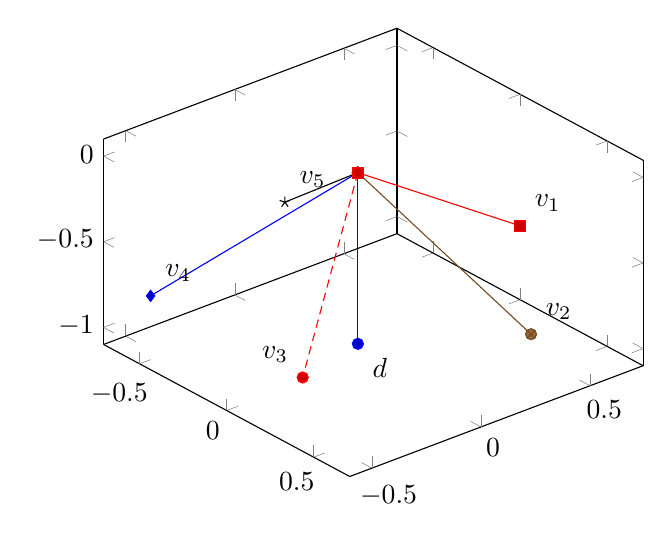
\begin{tikzpicture}
                  \begin{axis}[view = {50}{40}]
                        
                  \addplot3 coordinates 
                  {
                        (0,0,0)
                        (0,0,-1)
                  };

                  \node[below right, outer sep=2pt] at (0,0,-1) {$d$};

                  \addplot3 coordinates 
                  {
                        (0,0,0)
                        (0,0.74349606,-0.66874031)
                  };

                  \node[above right, outer sep=2pt] at (0,0.74349606,-0.66874031) {$v_{1}$};
                        
                  \addplot3 coordinates 
                  {
                        (0,0,0)
                        (0.70710677,0.22975292,-0.66874031)
                  };

                  \node[above right, outer sep=2pt] at (0.70710677,0.22975292,-0.66874031) {$v_{2}$};

                  \addplot3 coordinates 
                  {
                        (0,0,0)
                        (-0.70710677,0.22975292,-0.66874031)
                  };

                  \node[above right, outer sep=2pt] at (-0.70710677,0.22975292,-0.66874031) {$v_{5}$};

                  \addplot3 coordinates 
                  {
                        (0,0,0)
                        (-0.43701602,-0.60150095,-0.66874031)
                  };

                  \node[above right, outer sep=2pt] at (-0.43701602,-0.60150095,-0.66874031) {$v_{4}$};
                  
                  \addplot3 coordinates 
                  {
                        (0,0,0)
                        (0.43701602,-0.60150095,-0.66874031)
                  };

                  \node[above left, outer sep=2pt] at (0.43701602,-0.60150095,-0.66874031) {$v_{3}$};

                  \end{axis}
                        
            \end{tikzpicture}

      \end{proof}
\end{frame}

\begin{frame}
      \begin{proof}
            Let angle between $v_{1}, v_{3}$ and $v_{2}, v_{4}$ and $v_{3}, v_{5}$ and $v_{4}, v_{1}$ and $v_{5}, v_{2}$ be $\frac{\pi}{2}$.

            Then, the $5$ ribs of such an umbrella form an orthonormal representation of $C_{5}$.

            Let $d$ be the vector represent the handle, and $v_{1},v_{2},\dots,v_{5}$ be the $5$ ribs. And let $\gamma$ be the angle between the handle and any rib.

            So, by some calculation, we get
            \begin{eqnarray}
                  \theta(C_{5}) &=& \inf_{\{v_{1},v_{2} \hdots v_{5}\},c} \max_{i} \frac{1}{\langle c, v_{i} \rangle} \\
                  &\le& \max \frac{1}{<d,v_{i}>^{2}} \\
                  &=& \left(
                        \frac{1}{\cos(\gamma)}
                  \right)^{2} \\
                  &=& \sqrt{5}
            \end{eqnarray}
      \end{proof}
\end{frame}